\documentclass[a4paper]{article}
\usepackage{geometry}
\usepackage{graphicx}
\usepackage{natbib}
\usepackage{amsmath}
\usepackage{amssymb}
\usepackage{amsthm}
\usepackage{paralist}
\usepackage{epstopdf}
\usepackage{tabularx}
\usepackage{longtable}
\usepackage{multirow}
\usepackage{multicol}
\usepackage[hidelinks]{hyperref}
\usepackage{fancyvrb}
\usepackage{algorithm}
\usepackage{algorithmic}
\usepackage{float}
\usepackage{paralist}
\usepackage[svgname]{xcolor}
\usepackage{enumerate}
\usepackage{array}
\usepackage{times}
\usepackage{url}
\usepackage{fancyhdr}
\usepackage{comment}
\usepackage{environ}
\usepackage{times}
\usepackage{textcomp}
\usepackage{caption}
\usepackage{multirow}
\usepackage{bbm}

% \usepackage{kky}

\newcounter{thm}
\ifx\fact\undefined
\newtheorem{fact}[thm]{Fact}
\fi

\newcommand{\pen}{{\rm pen}}
\newcommand{\diag}{{\rm diag}}
\newcommand{\diam}{{\bf{\rm diam}}}
\newcommand{\spann}{{\bf{\rm span}}}
\newcommand{\nulll}{{\bf{\rm null}}}
% Distributions
\newcommand{\Bern}{{\bf{\rm Bern}}\,} % support of a function
\newcommand{\Categ}{{\bf{\rm Categ}}\,} % support of a function
\newcommand{\Mult}{{\bf{\rm Mult}}\,} % support of a function
\newcommand{\Dir}{{\bf{\rm Dir}}\,} % support of a function
\newcommand{\horizontalline}{\noindent\rule[0.5ex]{\linewidth}{1pt}}
\newcommand{\HRule}{\rule{\linewidth}{0.5mm}} 
\newcommand{\Hrule}{\rule{\linewidth}{0.3mm}}
\newcommand{\HRuleN}{\HRule\\} 
\newcommand{\HruleN}{\Hrule\\}
\newcommand{\superscript}[1]{{\scriptsize \ensuremath{^{\textrm{#1}}}}}
\newcommand{\supindex}[2]{#1^{(#2)}}
\newcommand{\xii}[1]{\supindex{x}{#1}}
\newcommand{\yii}[1]{\supindex{y}{#1}}
\newcommand{\zii}[1]{\supindex{z}{#1}}
\newcommand{\Xii}[1]{\supindex{X}{#1}}
\newcommand{\Yii}[1]{\supindex{Y}{#1}}
\newcommand{\Zii}[1]{\supindex{Z}{#1}}
\newcommand{\NN}{\mathbb{N}} % Natural numbers
\newcommand{\Ncal}{\mathcal{N}}
\newcommand{\Dcal}{\mathcal{D}}
\newcommand{\Lcal}{\mathcal{L}}
\newcommand{\Xcal}{\mathcal{X}}
\newcommand{\Pcal}{\mathcal{P}}
\newcommand{\Jcal}{\mathcal{J}}
\newcommand{\Rcal}{\mathcal{R}}
\newcommand{\indfone}{\mathbbm{1}}
\newcommand{\gb}{\mathbf{g}}
\newcommand{\Hb}{\mathbf{H}}
\newcommand{\Db}{\mathbf{D}}
\newcommand*{\zero}{{\bf 0}}
\newcommand*{\one}{{\bf 1}}

% Stuff mostly appearing in Statistics
\newcommand{\Xbar}{\bar{X}}
\newcommand{\Ybar}{\bar{Y}}
\newcommand{\Zbar}{\bar{Z}}
\newcommand{\Xb}{\mathbf{X}}


%%%%  brackets
\newcommand{\inner}[2]{\left\langle #1,#2 \right\rangle}
\newcommand{\rbr}[1]{\left(#1\right)}
\newcommand{\sbr}[1]{\left[#1\right]}
\newcommand{\cbr}[1]{\left\{#1\right\}}
\newcommand{\nbr}[1]{\left\|#1\right\|}
\newcommand{\abr}[1]{\left|#1\right|}

% derivatives and partial fractions
\newcommand{\differentiate}[2]{ \frac{ \ud #2}{\ud #1} }
\newcommand{\differentiateat}[3]{ \frac{ \ud #2}{\ud #1}  \Big|_{#1=#3} }
\newcommand{\partialfrac}[2]{ \frac{ \partial #2}{\partial #1} }
\newcommand{\partialfracat}[3]{ \frac{ \partial #2}{\partial #1} \Big|_{#1=#3} }
\newcommand{\partialfracorder}[3]{ \frac{ \partial^{#3} #2}{\partial^{#3} #1} }
\newcommand{\partialfracatorder}[4]{ \frac{ \partial^{#3} #2}{\partial^{#3} #1} \Big|_{#1=#4} }

\urlstyle{rm}

\setlength\parindent{0pt} % Removes all indentation from paragraphs
\theoremstyle{definition}
\newtheorem{definition}{Definition}[]
\newtheorem{conjecture}{Conjecture}[]
\newtheorem{example}{Example}[]
\newtheorem{theorem}{Theorem}[]
\newtheorem{lemma}{Lemma}
\newtheorem{proposition}{Proposition}
\newtheorem{corollary}{Corollary}


\floatname{algorithm}{Procedure}
\renewcommand{\algorithmicrequire}{\textbf{Input:}}
\renewcommand{\algorithmicensure}{\textbf{Output:}}
\newcommand{\abs}[1]{\lvert#1\rvert}
\newcommand{\norm}[1]{\lVert#1\rVert}
\newcommand{\RR}{\mathbb{R}}
\newcommand{\EE}{\mathbb{E}}
\newcommand{\PP}{\mathbb{P}}
\newcommand{\CC}{\mathbb{C}}
\newcommand{\Nat}{\mathbb{N}}
\newcommand{\br}[1]{\{#1\}}
\DeclareMathOperator*{\argmin}{arg\,min}
\DeclareMathOperator*{\argmax}{arg\,max}
\renewcommand{\qedsymbol}{$\blacksquare$}

\definecolor{dkgreen}{rgb}{0,0.6,0}
\definecolor{gray}{rgb}{0.5,0.5,0.5}
\definecolor{mauve}{rgb}{0.58,0,0.82}

\newcommand{\Var}{\mathrm{Var}}
\newcommand{\Cov}{\mathrm{Cov}}

\newcommand{\vc}[1]{\boldsymbol{#1}}
\newcommand{\xv}{\vc{x}}
\newcommand{\Sigmav}{\vc{\Sigma}}
\newcommand{\alphav}{\vc{\alpha}}
\newcommand{\muv}{\vc{\mu}}

\newcommand{\red}[1]{\textcolor{red}{#1}}

\def\x{\mathbf x}
\def\y{\mathbf y}
\def\w{\mathbf w}
\def\v{\mathbf v}
\def\E{\mathbb E}
\def\V{\mathbb V}

% TO SHOW SOLUTIONS, include following (else comment out):
\newenvironment{soln}{
    \leavevmode\color{blue}\ignorespaces
}{}

\hypersetup{
%    colorlinks,
    linkcolor={red!50!black},
    citecolor={blue!50!black},
    urlcolor={blue!80!black}
}

\geometry{
  top=1in,            % <-- you want to adjust this
  inner=1in,
  outer=1in,
  bottom=1in,
  headheight=3em,       % <-- and this
  headsep=2em,          % <-- and this
  footskip=3em,
}


\pagestyle{fancyplain}
\lhead{\fancyplain{}{Homework 5}}
\rhead{\fancyplain{}{CS 760 Machine Learning}}
\cfoot{\thepage}

\title{\textsc{Homework 5}} % Title

%%% NOTE:  Replace 'NAME HERE' etc., and delete any "\red{}" wrappers (so it won't show up as red)

\author{
Ryan Yee \\
9074025223\\
}

\date{}

\begin{document}

\maketitle 


\textbf{Instructions:}
Use this latex file as a template to develop your homework. We are changing our reproducibility policy on code submissions going forward. \textbf{Instead of uploading it on GitHub, please submit a separate zip file that contains your code. You will submit two files to Canvas, one is your pdf, and the other one is a zip file.} Late submissions may not be accepted. You can choose any programming language (i.e. python, R, or MATLAB). Please check Piazza for updates about the homework.
\vspace{0.1in}

This homework is more difficult than previous homework. The total amount of points for this homework is \textbf{150}. The extra credit reflects the level of difficulty.

\vspace{0.1in}

\section{Clustering}

\subsection{K-means Clustering (14 points)}

\begin{enumerate}

\item \textbf{(6 Points)}
Given $n$ observations $X_1^n = \{X_1, \dots, X_n\}$, $X_i \in \Xcal$, the K-means objective
is to find $k$
($<n$) centres $\mu_1^k = \{\mu_1, \dots, \mu_k\}$, and a rule $f:\Xcal \rightarrow
\{1,\dots, K\}$ so as to minimize the objective

\begin{equation}
J(\mu_1^K, f; X_1^n) = \sum_{i=1}^n \sum_{k=1}^K \indfone(f(X_i) = k) \|X_i - \mu_k\|^2
\label{eqn:kmeans}
\end{equation}

Let $\Jcal_K(X_1^n) = \min_{\mu_1^k, f} J(\mu_1^K, f; X_1^n)$. Prove that
$\Jcal_{K}(X_1^n)$ is a non-increasing function of $K$.

\item \textbf{(8 Points)}
Consider the K-means (Lloyd's) clustering algorithm we studied in class. We
terminate the algorithm when there are no changes to the objective.
Show that the algorithm terminates in a finite number of steps.

\end{enumerate}



\subsection{Experiment (20 Points)}

In this question, we will evaluate
K-means clustering and GMM on a simple 2 dimensional problem.
First, create a two-dimensional synthetic dataset of 300 points by sampling 100 points each from the
three Gaussian distributions shown below:
\[
P_a = \Ncal\left(
\begin{bmatrix}
-1 \\ -1
\end{bmatrix},
\;
\sigma\begin{bmatrix}
2, &0.5 \\ 0.5, &1
\end{bmatrix}
\right),
\quad
P_b = \Ncal\left(
\begin{bmatrix}
1 \\ -1
\end{bmatrix},
\;
 \sigma\begin{bmatrix}
1, &-0.5 \\ -0.5, &2
\end{bmatrix}
\right),
\quad
P_c = \Ncal\left(
\begin{bmatrix}
0 \\ 1
\end{bmatrix},
\;
 \sigma\begin{bmatrix}
1 &0 \\ 0, &2
\end{bmatrix}
\right)
\]
Here, $\sigma$ is a parameter we will change to produce different datasets.

\begin{itemize}
\item First implement K-means clustering and the expectation maximization algorithm for GMMs.
Execute both methods on five synthetic datasets,
generated as shown above with $\sigma \in \{0.5, 1, 2, 4, 8\}$. Finally, evaluate both methods on \emph{(i)} the clustering objective~\eqref{eqn:kmeans} and \emph{(ii)}  the clustering accuracy. For each of the two criteria, plot the value achieved by each method against $\sigma$.

\item Both algorithms are only guaranteed to find only a local optimum so we recommend trying multiple
restarts and picking the one with the lowest objective value (This is~\eqref{eqn:kmeans} for K-means and the negative log likelihood for GMMs).
You may also experiment with a smart initialization
strategy (such as kmeans++).

\item
To plot the clustering accuracy,  you may treat the `label' of points generated from distribution
$P_u$ as $u$, where $u\in \{a, b, c\}$.
Assume that the cluster id $i$ returned by a method is $i\in \{1, 2, 3\}$.
Since clustering is an unsupervised learning problem, you should obtain the best possible mapping
from $\{1, 2, 3\}$ to $\{a, b, c\}$ to compute the clustering objective.
One way to do this is to compare the clustering centers returned by the method (centroids for
K-means, means for GMMs) and map them to the distribution with the closest mean.

\end{itemize}

Points break down: 7 points each for implementation of each method, 6 points for reporting of
evaluation metrics.

\section{Linear Dimensionality Reduction}

\subsection{Principal Components Analysis  (10 points)}
\label{sec:pca}

Principal Components Analysis (PCA) is a popular method for linear dimensionality reduction. PCA attempts to find a lower dimensional subspace such that when you project the data onto the subspace as much of the information is preserved. Say we have data $X = [x_1^\top; \dots; x_n^\top] \in \RR^{n\times D}$ where  $x_i \in \RR^D$. We wish to find a $d$ ($ < D$) dimensional subspace $A = [a_1, \dots, a_d] \in \RR^{D\times d}$, such that $ a_i \in \RR^D$ and $A^\top A = I_d$, so as to maximize $\frac{1}{n} \sum_{i=1}^n \|A^\top x_i\|^2$.
\begin{enumerate}

\item  \textbf{(4 Points)}
Suppose we wish to find the first direction $a_1$ (such that $a_1^\top a_1 = 1$) to maximize $\frac{1}{n} \sum_i (a_1^\top X_i)^2$.
Show that $a_1$ is the first right singular vector of $X$.

\begin{soln}
  Let $a_1$ be the first right singular vector of $X$.
  Then $X^T X a_1 = \lambda_1 a_1$ where $\lambda_1$ is an eigenvalue of $X^T X$ and $\lambda_1 \geq \lambda_i$ for $i = 2, 3, \dots, D$ by definition.
  Then:
  $$ X^T X a_1 = \lambda_1 a_1 $$
  $$ a_1^T X^T X a_1 = \lambda_1 a_1^T a_1 $$
  $$ \sum_i (a_1^\top X_i)^2 = \lambda_1 $$
  Since $\lambda_1$ is the largest eigenvalue of $X^T X$, the function is maximized if $a_1$ is a right singular vector of $X$.
  $a_1$ must be a right singular vector of $X$ for the equation to hold.
  Thus, the function is maximized when $a_1$ is the first right singular vector of $X$.
\end{soln}

\item  \textbf{(6 Points)}
Given $a_1, \dots, a_k$, let $A_k = [a_1, \dots, a_k]$ and 
$\tilde{x}_i = x_i - A A^\top x_i$. We wish to find $a_{k+1}$, to maximize
$\frac{1}{n} \sum_i (a_{k+1}^\top \tilde{x}_i)^2$. Show that $a_{k+1}$ is the
$(k+1)^{th}$ right singular vector of $X$.

\begin{soln}
  In matrix form, we have $\tilde{X} = X - XAA^T$ since $AA^T$ is symmetric.
  Then:
  $$ 
  \begin{aligned}
    \tilde{X}^T \tilde{X} & = (X - XAA^T)^T (X - XAA^T) \\
    & = X^TX -X^TXAA^T - AA^TX^TX + AA^TX^TXAA^T \\
  \end{aligned}
  $$
  So:
  $$
  \begin{aligned}
    \tilde{X}^T \tilde{X} A & = (X^TX -X^TXAA^T - AA^TX^TX + AA^TX^TXAA^T) A \\
    & = X^TXA - X^TXA - AA^TX^TXA + AA^TX^TXA \\
    & = \mathbf{0}
  \end{aligned}
  $$
  So $a_1, \dots, a_k$ do not maximize $\sum_i (a_{k+1}^\top \tilde{x}_i)^2 = a_{k+1}^T \tilde{X}^T \tilde{X} a_{k+1}$. 
  Now consider $a^*$ which is any singular vector of $X$ that is not in $A$.
  Then:
  $$
  \begin{aligned}
    \tilde{X}^T \tilde{X} a^* & = (X^TX -X^TXAA^T - AA^TX^TX + AA^TX^TXAA^T) a^* \\
    & = X^TXa^* \\
    & = \lambda^* a^*
  \end{aligned}
  $$
  since $a^*$ is orthogonal to all the vectors in $A$.
  Therefore, $a_{k+1}$ is the first right singular vector of $\tilde{X}$.
  So by the arguments in (1), the function is maximized when $a_{k+1}$ is the $(k+1)^{th}$ singular vector of $X$.
\end{soln}



% \item \textbf{(2 Points)}
% You are given a point $z_*$ in the $d$ dimensional space obtained using PCA.
% What is $x_*$, the reconstruction of $z_*$ in the original $D$ dimensional space?



\end{enumerate}


\subsection{Dimensionality reduction via optimization (22 points)}

We will now motivate the dimensionality reduction problem from a slightly different
perspective. The resulting algorithm has many similarities to PCA.
We will refer to method as DRO.

As before, you are given data $\{x_i\}_{i=1}^n$, where $x_i \in \RR^D$. Let $X=[x_1^\top; \dots
x_n^\top] \in \RR^{n\times D}$. We suspect that the data
actually lies approximately in  a $d$ dimensional affine subspace.
Here $d<D$ and $d<n$.
Our goal, as in PCA, is to use this dataset to find a $d$ dimensional representation $z$ for each $x\in\RR^D$.
(We will assume that the span of the data has dimension larger than
$d$, but our method should work whether $n>D$ or $n<D$.)


Let $z_i\in \RR^d$ be the lower dimensional representation for $x_i$ and
let $Z = [z_1^\top; \dots; z_n^\top] \in \RR^{n\times d}$.
We wish to find parameters $A \in \RR^{D\times d}$, $b\in\RR^D$ and the lower
dimensional representation $Z\in \RR^{n\times d}$ so as to minimize 
\begin{equation}
J(A,b,Z) = \frac{1}{n} \sum_{i=1}^n \|x_i - Az_i - b\|^2 = \| X - ZA^\top - \one b^\top\|_F^2.
\label{eqn:dimobj}
\end{equation}
Here, $\|A\|^2_F = \sum_{i,j} A_{ij}^2$ is the Frobenius norm of a matrix.


\begin{enumerate}
\item \textbf{(3 Points)}
Let $M\in\RR^{d\times d}$ be an arbitrary invertible matrix and $p\in\RR^{d}$ be an arbitrary vector.
Denote, $A_2 = A_1M^{-1}$, $b_2 = b_1- A_1M^{-1}p$ and $Z_2 = Z_1 M^\top +
\one p^\top$.
Show that both
$(A_1, b_1, Z_1)$ and $(A_2, b_2, Z_2)$ achieve the same objective value $J$~\eqref{eqn:dimobj}.
\end{enumerate}

\begin{soln}
  $$
  \begin{aligned}
    J & = \| X - Z_2A_2^\top - \one b_2^\top \| \\
    & = \| X - (Z_1 M^\top + \one p^\top)(A_1M^{-1})^\top - \one (b_1- A_1M^{-1}p)^\top \| \\
    & = \| X - Z_1 M^\top M^{-\top}A_1^\top - \one p^\top M^{-\top}A_1^\top - \one b_1^\top + \one p^\top M^{-\top}A_1^\top \| \\
    & = \| X - Z_1A_1^\top - \one b_1^\top \|
  \end{aligned}
  $$
\end{soln}

Therefore, in order to make the problem determined, we need to impose some
constraint on $Z$. We will assume that the $z_i$'s have zero mean and identity covariance.
That is,
\begin{align*}
\Zbar = \frac{1}{n} \sum_{i=1}^n z_i =\frac{1}{n} Z^\top {\bf 1}_d = 0, \hspace{0.3in} 
S = \frac{1}{n} \sum_{i=1}^n z_i z_i^\top 
= \frac{1}{n} Z Z^\top
= I_d
\end{align*}
Here, ${\bf 1}_d = [1, 1 \dots, 1]^\top \in\RR^d$ and $I_d$  is the $d\times d$ identity matrix.

\begin{enumerate}
\setcounter{enumi}{1}
\item \textbf{(16 Points)}
Outline a procedure to solve the above problem. Specify how you
would obtain $A, Z, b$ which minimize the objective and satisfy the constraints.

\textbf{Hint: }The rank $k$ approximation of a matrix in Frobenius norm is obtained by
taking its SVD and then zeroing out all but the first $k$ singular values.

\begin{soln}
  Note that in the best case $X - ZA^\top - \one b^\top = 0$.
  First, solve for $b$:
  \begin{gather*}
    X - ZA^\top - \one b^\top = 0 \\
    X - ZA^\top = \one b^\top \\
    X^\top - AZ^\top = b \one^\top \\
    X^\top \one - AZ^\top \one = b n \\
    \frac{1}{n} X^\top \one = b \\
    \frac{1}{n} \sum_{i=1}^{n} x_i = b 
  \end{gather*}
  Next, find $Q=ZA^\top$:
  \begin{gather*}
    X - Q - \one b^\top = 0 \\
    Q = X - \one b^\top
  \end{gather*}
  Note that the rows of $Q$ have mean zero.
  Using the \textit{hint} from above, the rank $k$ approximation of $Q$ is its SVD with all but the first $k$ singular values singled out.
  So, let $A_k = [a_1, \dots, a_k]$ where $a_i$ is the $i$th right singular vector of $Q$.

\end{soln}

\item \textbf{(3 Points)}
You are given a point $x_*$ in the original $D$ dimensional space.
State the rule to obtain the $d$ dimensional
representation $z_*$ for this new point.
(If $x_*$ is some original point $x_i$ from the $D$--dimensional space, it shoud be the
$d$--dimensional representation $z_i$.)

\begin{soln}
  $z_i = A^\top (x_i - b)$
\end{soln}

%\item \textbf{(1 Point)}
% You are given a point $z_*$ in the $d$ dimensional space obtained using DRO.
% What is $x_*$, the reconstruction of $z_*$ in the original $D$ dimensional space?

\end{enumerate}


\subsection{Dimensionality reduction via a generative model (42 points)}

We will now study dimensionality reduction via a generative model.
We will refer to method as DRLV.
We will assume a $d (<n)$ dimensional latent space and
the following generative process for the data.
\begin{align*}
& z \sim \Ncal(\zero, I),  \quad  z\in \RR^d \\
& x|z \sim \Ncal(Az + b, \eta^2 I),  \quad  x\in \RR^D 
\end{align*}
The model says that we first sample a $d$ dimensional Gaussian with zero mean
and identity variance. Then we map it to $D$ dimensions by computing $Az+b$.
Finally, we add some spherical Gaussian noise with variance $\eta^2$ on each
dimension.

We will use an expectation maximization (EM)
procedure to learn the parameters $A, b, \eta$. So far we have only studied
 EM with discrete latent variables. In this problem, we will look at
EM with a continuous latent variable which has a parametric distribution.
The following results will be useful.\\

\begin{fact}[Conditional of a Gaussian]
Say $(Y_1, Y_2), Y_i \in \RR^{d_i}$ is Gaussian distributed.
\[
\left(\begin{array}{c}Y_1 \\ Y_2\end{array}\right) =
\Ncal \left( \left(\begin{array}{c} \mu_1 \\ \mu_2 \end{array} \right), 
\left[ \begin{array}{cc} \Sigma_{11} & \Sigma_{12} \\ \Sigma_{12}^\top &
  \Sigma_{22} \end{array} \right] 
  \right)
\]
Then, conditioned on $Y_1 = y_1$ the distribution for $Y_2$ is
\[
Y_2 | Y_1 = y_1 \sim \Ncal(\mu_2+ \Sigma_{12}^\top \Sigma_{11}^{-1} (y_1 - \mu_1), \;
  \Sigma_{22} - \Sigma_{12}^\top \Sigma_{11}^{-1}\Sigma_{12} )
\]
\end{fact}

\begin{fact}[Some Matrix Derivatives]
Let $X\in \RR^{r\times c}$, and $u\in \RR^r$, $v,w \in \RR^c$.
\begin{align*}
\nabla_X v^\top X^\top u &= uv^\top \\
\nabla_X v^\top X^\top X w &= X(vw^\top + wv^\top)
\end{align*}
\end{fact}
\vspace{0.1in}

\begin{enumerate}
\item \textbf{(10 Points)}
Assuming some given values for $A$, $b$, and $\eta^2$, write down the joint distribution of $(z,x)$. Use this to derive the marginal
distribution of $x$ and the conditional distribution $z|x$. 

\begin{soln}
  $$
  \begin{aligned}
    \mathbbm{P}(x, z) & = \mathbbm{P}(x \vert z) \mathbbm{P}(z) \\
    & = (2 \pi)^{-D/2} \det(\eta^2 I)^{-1/2} \exp\left\{-\frac{1}{2} (x - Az -  b)^\top (\eta^2 I)^{-1} (x - Az -b) \right\} (2 \pi)^{-d/2} \exp\left\{ -\frac{1}{2} z^\top z\right\} \\
    & = (2 \pi)^{-\frac{D + d}{2}} \det(\eta^2 I)^{-1/2} \exp\left\{-\frac{1}{2} \left((x - Az -  b)^\top (\eta^2 I)^{-1} (x - Az -b) + \eta^2 z^\top z\right) \right\}
    % & = (2 \pi)^{-\frac{D + d}{2}} \det(\eta^2 I)^{-1/2} \exp\left\{-\frac{1}{2 \eta^2} (x^\top x - (Az+b)^\top x - x^\top (Az+b) + (Az+b)^\top (Az+b) + \eta^2 z^\top z) \right\} \\
    % & = 
  \end{aligned}
  $$

  We can assume $x$ follows a Gaussian distribution. 
  It is straightforward to see $\mathbbm{E}[X] = b$.
  Then 
  $$
  \begin{aligned}
    \text{Var}(X) & = \mathbbm{E}[(X-b) (X-b)^\top] \\
    & = \mathbbm{E}[(AZ + \epsilon) (AZ + \epsilon)^\top] \\
    & = \mathbbm{E}[AZZ^\top A^\top +2 AZ \epsilon^\top + \epsilon \epsilon^\top] \\
    & = AA^\top + \eta^2 I
  \end{aligned}
  $$
  So, $x \sim \Ncal(b, A^\top A + \eta^2 I)$.
  Then:
  $$
  \begin{aligned}
    Cov(x, z) & = \mathbbm{E}[X^\top Z] \\
    & = \mathbbm{E}[(AZ + b + \epsilon)^\top Z] \\
    & = \mathbbm{E}[Z^\top A^\top Z + b^\top Z + \epsilon^\top Z] \\
    & = A^\top
  \end{aligned}
  $$
  Using \textbf{Fact 1} we have $z \vert x \sim \Ncal(A(AA^\top + \eta^2 I)^{-1}(x-b), I - A(AA^\top + \eta^2 I)^{-1}A^\top)$
\end{soln}

\item \textbf{(4 points)}
Write the log likelihood in terms of parameters $A$, $b$, and $\eta^2$.

\begin{soln}
  $\mathcal{L}(A, b, \eta^2) = \sum_{i=1}^{n} -\frac{D}{2} \log(2 \pi) -\frac{1}{2} \log(\det(AA^\top + \eta^2 I)) -\frac{1}{2} (x-b)^\top (AA^\top + \eta^2 I)^{-1} (x-b)$
\end{soln}

\item \textbf{(4 Points)}
First obtain the Maximum Likelihood Estimate for $b$. This does not require EM.

\begin{soln}
  $$
  \begin{aligned}
    \frac{\partial \mathcal{L}}{\partial b} & = \sum_{i=1}^{n} \frac{\partial}{\partial b} \left[-\frac{1}{2} (x-b)^\top (AA^\top + \eta^2 I)^{-1} (x-b)\right] \\
    & = -\frac{1}{2} \sum_{i=1}^{n} \frac{\partial}{\partial b} \left[b^\top (AA^\top + \eta^2 I)^{-1} b - 2b^\top(AA^\top + \eta^2 I)^{-1}x \right] \\
    & = -\frac{1}{2} \sum_{i=1}^{n} \left[2 (AA^\top + \eta^2 I)^{-1} b - 2(AA^\top + \eta^2 I)^{-1}x \right] \\
  \end{aligned}
  $$
  Setting $\frac{\partial \mathcal{L}}{\partial b} = 0$:
  \begin{gather*}
    (AA^\top + \eta^2 I)^{-1} bn = (AA^\top + \eta^2 I)^{-1} \sum_{i=1}^{n} x_i \\
    b = \frac{1}{n} \sum_{i=1}^{n} x_i
  \end{gather*}
\end{soln}

\item \textbf{(10 Points)}
To apply the EM algorithm,
let $Q(z_i)$  denote some distribution over $z_i$ for each $z_i$.
Obtain a lower bound on the log likelihood via Jensen's inequality.

\begin{soln}
  $$
  \begin{aligned}
    \mathcal{L}(A, b, \eta^2) & = \sum_{i=1}^{n} \log\left(\sum_{j=1}^{k} Q(z_j) \frac{p(x_i, z_j)}{Q(z_j)} \right) \\
    & \geq \sum_{i=1}^{n} \sum_{j=1}^{k} Q(z_j) \log\left(\frac{p(x_i, z_j)}{Q(z_j)}\right)
  \end{aligned}
  $$
\end{soln}

\item \textbf{(4 Points)}
Recall, from the lectures, that we chose
$Q(z_i) =  \PP(z_i|x_i)$ in the E-step to obtain the tightest
possible lower bound for the log likelihood.
Here, $ \PP(z_i|x_i)$ is the conditional distribution of $z_i$
given $x_i$ under the current estimates for $A$, $b$, and $\eta$.
Write down the E-step update for the next iteration. \\
N.B: Unlike in GMMs, where the latent variable was discrete, here the latent variable is continuous. Fortunately, it has a parametric form we can represent $Q(z_i)$ using a finite number of parameters. \\
(Hint: See part 1)

\begin{soln}
  \begin{gather*}
    w^{(i)}_j = \mathbb{P}(z_i = j \vert x_i; A, b, \eta^2) \\
    w^{(i)} \sim \Ncal(A(AA^\top + \eta^2 I)^{-1}(x_i-b), I - A(AA^\top + \eta^2 I)^{-1}A^\top)
  \end{gather*}
  So we can calculate $w^{(i)}_j$ for any $j$.
\end{soln}

\item \textbf{(10 Points)}
Now write down the M-step update for parameters $A$ and $\eta$, obtained
by maximizing the lower bound obtained from parts 3 and 4.

\begin{soln}
  $$
  \begin{aligned}
    \mathcal{L}(A, b, \eta^2; X, Z) & = \log p(X \vert Z) + \log p(z) \\
    & = -\frac{1}{2} \left[-2\log(\det(\eta^2 I)^{-1}) + (X-AZ-b)^\top (\eta^2 I)^{-1} (X-AZ-b)+Z^\top Z\right]
  \end{aligned}
  $$
  To maximize $A$:
  $$
  \begin{aligned}
    \frac{\partial \mathcal{L}}{\partial A} & = -\frac{1}{2} \frac{\partial}{\partial A} \left[(X-AZ-b)^\top (\eta^2 I)^{-1} (X-AZ-b)\right] \\
    & = -\frac{1}{2} \frac{\partial}{\partial A} \left[-2 Z^\top A^\top (\eta^2 I)^{-1}(X-b) + Z^\top A^\top AZ \right] \\
    & = (\eta^2 I)^{-1}(X-b)Z^\top - A(ZZ^\top) \\
  \end{aligned}
  $$
  Set $\frac{\partial \mathcal{L}}{\partial A} = 0$:
  $$
  \begin{aligned}
    A(ZZ^\top) & = (\eta^2 I)^{-1}(X-b)Z^\top \\
    A & = (\eta^2 I)^{-1}(X-b)Z^\top (ZZ^\top)^{-1}
  \end{aligned}
  $$
  To maximize $\eta^2$:
  $$\frac{\partial \mathcal{L}}{\partial \eta^2} = -\frac{1}{\eta^2} + \frac{1}{2 (\eta^2)^2}(X-AZ-b)^\top(X-AZ-b)$$
  Set $\frac{\partial \mathcal{L}}{\partial \eta^2} = 0$:
  $$
  \begin{aligned}
    \frac{1}{\eta^2} & = \frac{1}{2 (\eta^2)^2}(X-AZ-b)^\top(X-AZ-b) \\
    \eta^2 & = (X-AZ-b)^\top(X-AZ-b)
  \end{aligned}
  $$
\end{soln}

% \item \textbf{(2 Points)}
% You are given a point $x_*$ in the original $D$ dimensional space.
% We will use the posterior mean of $z_*|x_*$ as the $d$ dimensional
% representation for this new point.
% State the rule (equation) to compute this.

% \item \textbf{(1 Points)}
% You are given a point $z_*$ in the $d$ dimensional space obtained using DRLV.
% What is $x_*$, the reconstruction of $z_*$ in the original $D$ dimensional space?

\end{enumerate}

 
\subsection{Experiment (42 points)}

Here we will compare the above three methods on two data sets. 

\begin{itemize}
\item We will implement three variants of PCA:
\begin{enumerate}
    \item "buggy PCA": PCA applied directly on the matrix $X$.
    \item "demeaned PCA": We subtract the mean along each dimension before applying PCA.
    \item "normalized PCA": Before applying PCA, we subtract the mean and scale each dimension so that the sample  mean and standard deviation along each dimension is $0$ and $1$ respectively.
    
\end{enumerate}



\item 
One way to study how well the low dimensional representation $Z$ captures the linear
structure in our data is to project $Z$ back to $D$ dimensions and look at the reconstruction
error. For PCA, if we mapped it to $d$ dimensions via $z = Vx$ then the
reconstruction is $V^\top z$. For the preprocessed versions, we first do this and then
reverse the preprocessing steps as well. For DRO  we just compute $Az + b$.
For DRLV, we will use the posterior mean $\EE[z|x]$ as the lower dimensional
representation and $Az + b$ as the reconstruction. \\
We will compare all four methods by the reconstruction error on the datasets.

\item 
Please implement code for the five methods: Buggy PCA (just take the SVD of $X$)
, Demeaned PCA,
Normalized PCA, DRO, DRLV. In all cases your function should take in
an $n \times d$ data matrix and $d$ as an argument. It should return the
the $d$ dimensional representations, the estimated parameters, and the
reconstructions of these representations in $D$ dimensions. 
For DRLV, use the values obtained from DRO as initializations for $A$. Set $\eta$
based on the reconstruction errors of DRO.
Use $10$ iterations of EM.

\item
You are given two datasets: A two Dimensional dataset with $50$ points 
\texttt{data2D.csv} and a thousand dimensional dataset with $500$ points
\texttt{data1000D.csv}. 

\item
For the $2D$ dataset use $d=1$. For the $1000D$ dataset, you need to choose
$d$. For this, observe the singular values in DRO and see if there is a clear
``knee point" in the spectrum.
Attach any figures/ Statistics you computed to justify your choice.

\item
For the $2D$ dataset you need to attach the a 
plot comparing the orignal points with the reconstructed points for all five
methods.
For both datasets you should also report the reconstruction errors, that is the squared sum of
differences $\sum_{i=1}^n \|x_i - r(z_i)\|^2$,
where $x_i$'s are the original points and $r(z_i)$ are the $D$ dimensional points
reconstructed from the 
$d$ dimensional representation $z_i$.

\begin{soln}

  % 2D Visualizations
  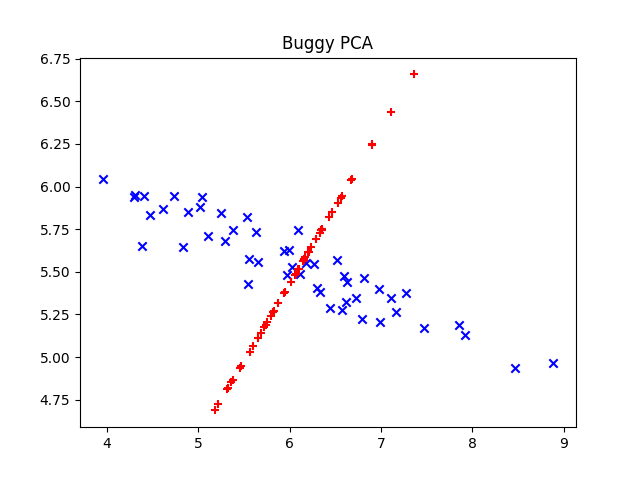
\includegraphics[width=3in]{../figs/buggy_pca.png} \hspace{0.1in}
  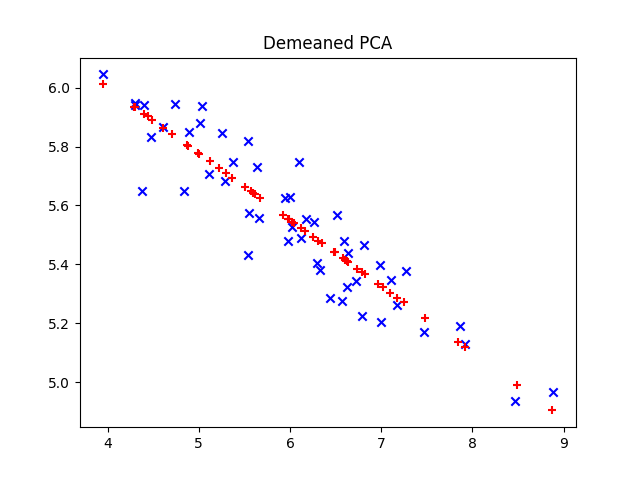
\includegraphics[width=3in]{../figs/demeaned_pca.png} \\
  \begin{center}
    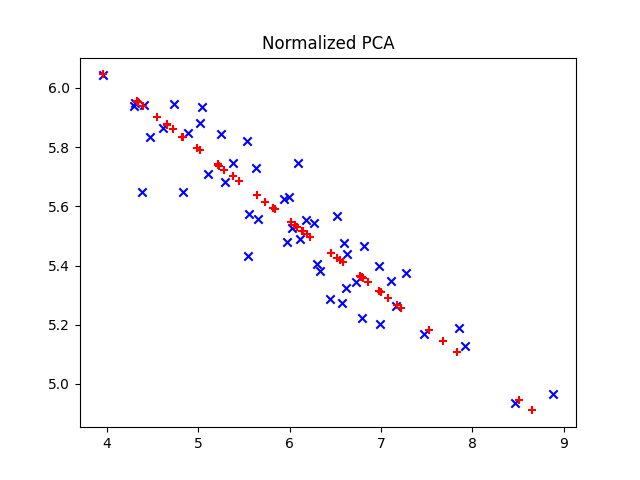
\includegraphics[width=3in]{../figs/normalized_pca.png}
  \end{center}
  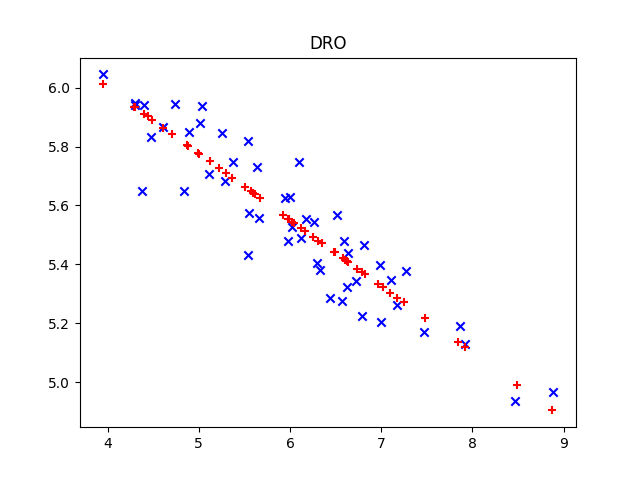
\includegraphics[width=3in]{../figs/dro.png}
  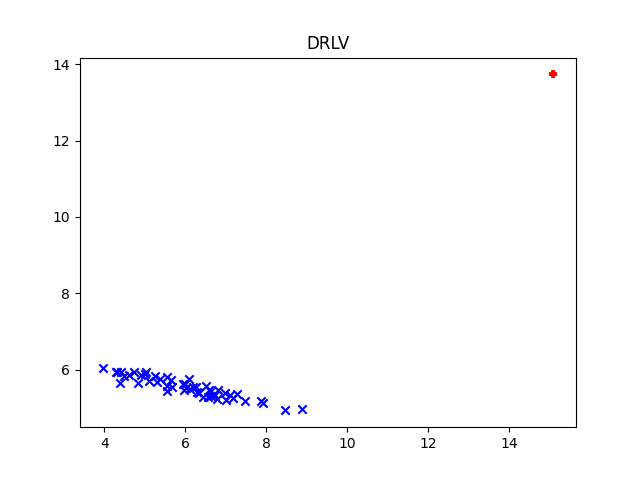
\includegraphics[width=3in]{../figs/drlv.png}

  % 2D Data Reconstruction Error
  \begin{center}
    \textbf{2D Data} \\
    \begin{tabular}{ c  c }
      \hline
      Method & Reconstruction Error \\ \hline
      Buggy PCA & 0.886903 \\
      Demeaned PCA & 0.010006 \\
      Normalized PCA & 0.049472 \\
      DRO & 0.010006 \\
      DRLV & 150.738297 \\
      \hline
    \end{tabular}
  \end{center}

  % 1000D Error Curves
  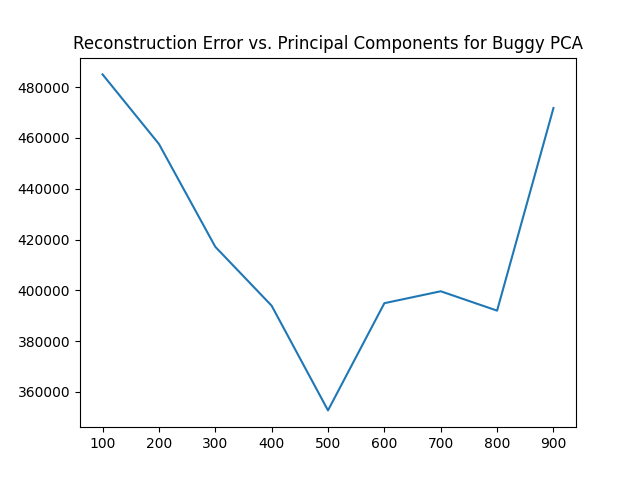
\includegraphics[width=3in]{../figs/buggy_error_curve.png} \hspace{0.1in}
  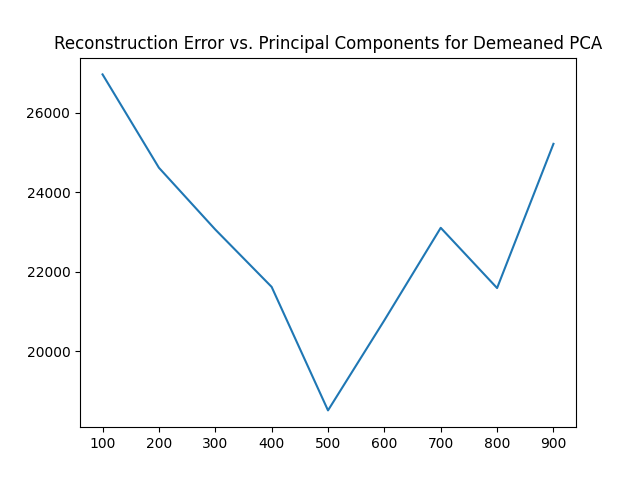
\includegraphics[width=3in]{../figs/demeaned_error_curve.png} \\
  \begin{center}
    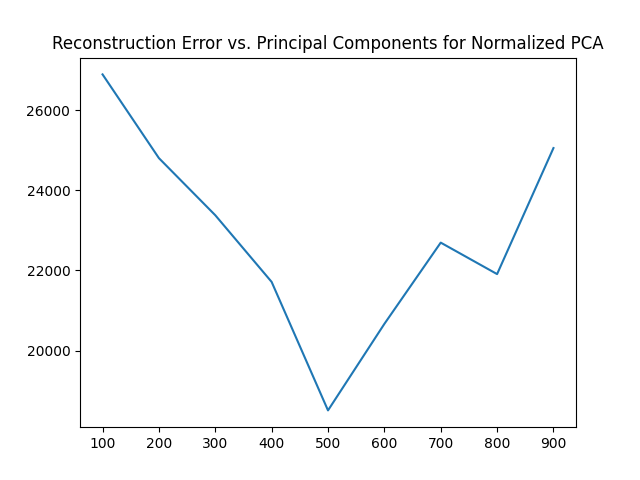
\includegraphics[width=3in]{../figs/normalized_error_curve.png}
  \end{center} 

  The ``knee-point'' seems to be at $d = 500$ for all the PCA methods.
  This makes sense, because there are 500 observations in the 1000D data ($n=500$), which means its SVD has 500 singular values.
  I will use $d=500$ for all the methods.

  % 1000D Data Reconstruction Error
  \begin{center}
    \textbf{1000D Data} \\
    \begin{tabular}{ c  c }
      \hline
      Method & Reconstruction Error \\ \hline
      Buggy PCA & 352741 \\
      Demeaned PCA & 18509 \\
      Normalized PCA & 18503 \\
      DRO & 18509 \\
      DRLV & 1103133\\
      \hline
    \end{tabular}
  \end{center}
  There is definitely issues with my DRLV implementation.
  I'm not sure if it's the derivations or the implementation to be completely honest.
\end{soln}

\item \textbf{Questions:} After you have completed the experiments, please answer the following questions.
\begin{enumerate}
\item Look at the results for Buggy PCA. The reconstruction error is bad and the
reconstructed points don't seem to well represent the original points. Why is
this? \\
\textbf{Hint: } Which subspace is Buggy PCA trying to project the points
onto?

\begin{soln}
  Buggy PCA is trying to project onto a subspace that passes through the origin.
  In the other PCA methods, we account for this by subtracting the mean from each dimension so the mean of each dimension is zero.
\end{soln}

\item The error criterion we are using is the average squared error 
between the original points and the reconstructed points.
In both examples DRO and demeaned PCA achieves the lowest error among all
methods. 
Is this surprising? Why?

\begin{soln}
  This is not surprising.
  Demeaned PCA is equivalent to DRO.
  In problem 2.2, we derived DRO such that the reconstruction error was minimized.
\end{soln}

\end{enumerate}

\item Point allocation:
\begin{itemize}
\item Implementation of the three PCA methods: \textbf{(10 Points)}
\item Implementation of DRO and DRLV: \textbf{(20 points)}
\item Implementing reconstructions and reporting results: \textbf{(5 points)}
\item Choice of $d$ for $1000D$ dataset and appropriate justification:
\textbf{(3 Points)}
\item Questions \textbf{(4 Points)}
\end{itemize}

\end{itemize}


%\vspace{0.1in}

\textbf{Partial answers:}
These were our errors on all methods for the $2D$ dataset and the reconstructions obtained for Buggy PCA and Demeaned PCA.
We have provided them to cross-check with your solution.
Our implementation may have bugs so if your answer does not tally, first double check with your peers and then speak to the TA/Instrutor.
\begin{verbatim}
Reconstruction Errors:
Buggy PCA: 0.886903
Demeaned PCA: 0.010006
Normalized PCA: 0.049472
DRO: 0.010006
DRLV: 0.010081
\end{verbatim}

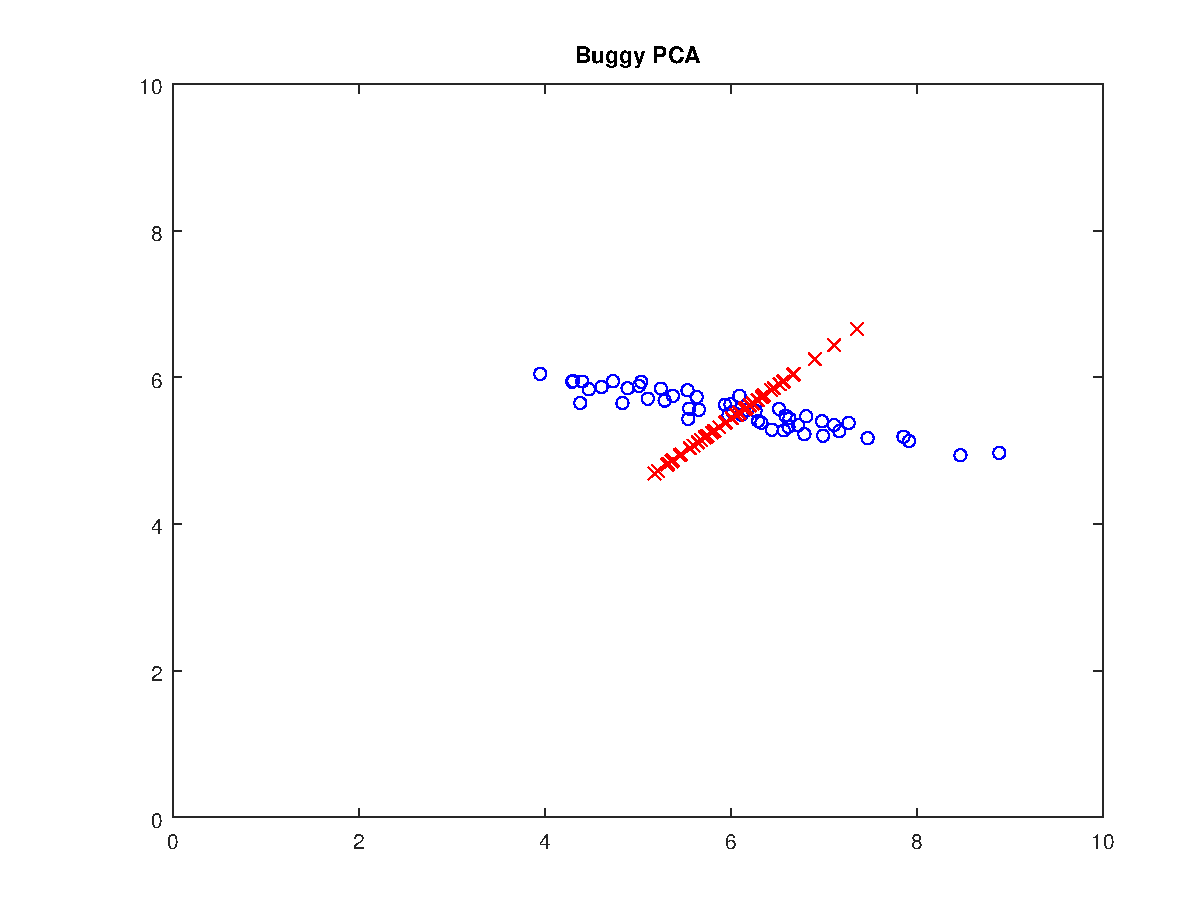
\includegraphics[width=3in]{pcaprog/buggy_pca} \hspace{0.4in}
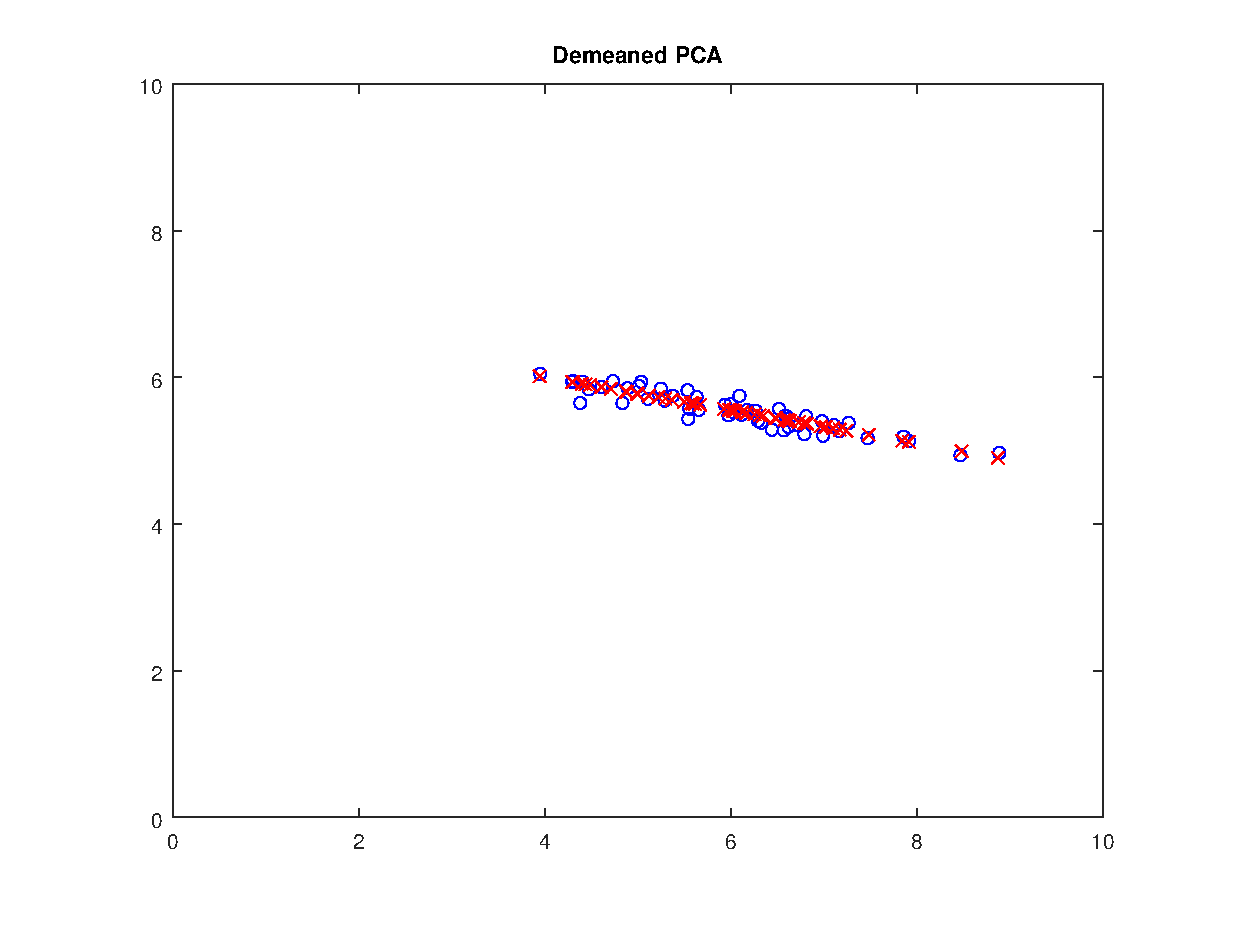
\includegraphics[width=3in]{pcaprog/demeaned_pca} \\
The blue circles are from the original dataset and the red crosses are the reconstructed points.

\vspace{0.2in}





\bibliographystyle{apalike}
\end{document}


